\documentclass{ieeeaccess}
%Adjusted 05/13/2026 at the byline author names
\usepackage{cite}
\usepackage{amsmath,amssymb,amsfonts}
\usepackage{algorithmic}
\usepackage{graphicx}
\usepackage{textcomp}

\usepackage{bm}
\makeatletter
\AtBeginDocument{\DeclareMathVersion{bold}
\SetSymbolFont{operators}{bold}{T1}{times}{b}{n}
\SetSymbolFont{NewLetters}{bold}{T1}{times}{b}{it}
\SetMathAlphabet{\mathrm}{bold}{T1}{times}{b}{n}
\SetMathAlphabet{\mathit}{bold}{T1}{times}{b}{it}
\SetMathAlphabet{\mathbf}{bold}{T1}{times}{b}{n}
\SetMathAlphabet{\mathtt}{bold}{OT1}{pcr}{b}{n}
\SetSymbolFont{symbols}{bold}{OMS}{cmsy}{b}{n}
\renewcommand\boldmath{\@nomath\boldmath\mathversion{bold}}}
\makeatother

\def\BibTeX{{\rm B\kern-.05em{\sc i\kern-.025em b}\kern-.08em
    T\kern-.1667em\lower.7ex\hbox{E}\kern-.125emX}}

%增加公式定义
\newcommand{\Pre}{\mathrm{Pre}}  % 或者 \mathcal{P}

\usepackage{tabularx}  % 需在导言区添加（如果尚未加载）
\newcolumntype{C}{>{\centering\arraybackslash}X}   % 居中自动宽度列


%Your document starts from here ___________________________________________________
\begin{document}
\history{Date of publication xxxx 00, 0000, date of current version xxxx 00, 0000.}
\doi{10.1109/ACCESS.2024.0429000}

\title{A Virtual-Real Integrated Intelligent Learning System for Complex Mechanical Engineering: Design, Implementation, and Performance Evaluation}
\author{\uppercase{First A. Author}\authorrefmark{1}, \IEEEmembership{Fellow, IEEE},
\uppercase{Second B. Author}\authorrefmark{2}, AND \uppercase{Third C. Author},
Jr.\authorrefmark{3},
\IEEEmembership{Member, IEEE}}

\address[1]{National Institute of Standards and
Technology, Boulder, CO 80305 USA (e-mail: author@boulder.nist.gov)}
\address[2]{Department of Physics, Colorado State University, Fort Collins,
CO 80523 USA (e-mail: author@lamar.colostate.edu)}
\address[3]{Electrical Engineering Department, University of Colorado, Boulder, CO
80309 USA}
\tfootnote{This paragraph of the first footnote will contain support
information, including sponsor and financial support acknowledgment. For
example, ``This work was supported in part by the U.S. Department of
Commerce under Grant BS123456.''}

\markboth
{Author \headeretal: Preparation of Papers for IEEE TRANSACTIONS and JOURNALS}
{Author \headeretal: Preparation of Papers for IEEE TRANSACTIONS and JOURNALS}

\corresp{Corresponding author: First A. Author (e-mail: author@ boulder.nist.gov).}


\begin{abstract}
This paper presents the design, implementation, and performance evaluation of a virtual-real integrated intelligent learning system for complex mechanical engineering. 
The system addresses three key engineering challenges: (i) isolation of front-end simulation logs from back-end reasoning, (ii) lack of semantic constraints in learning path recommendation, and (iii) high-concurrency bottlenecks of monolithic architectures. A microservice topology (Vue3 + Golang + Python + Neo4j) is constructed to achieve millisecond-level log ingestion and state update. A knowledge graph of mechanical principles (247 nodes, 180k+ real-world interaction logs) is built, and an improved KG-A* algorithm is proposed, which enforces prerequisite dependencies as hard pruning constraints to guarantee engineering-compliant path planning. Experimental results on the MechKG-2024 dataset show that KG-A* outperforms baseline models in knowledge state prediction (AUC: 0.847) and path recommendation (HR@5: 0.687). Stress tests under 500 concurrent requests yield an average response time below 120 ms and a throughput of ~3890 QPS, demonstrating enterprise-grade robustness. The system provides a deployable solution for digital twin-based engineering training platforms.
\end{abstract}

\begin{keywords}
Knowledge Graph, Microservices Architecture, Digital Twin, Adaptive Pathfinding, Improved A* Algorithm.
\end{keywords}

\titlepgskip=-21pt

\maketitle

\section{Introduction}
\label{sec:introduction}

\subsection{Background and Challenges}
The rapid development of industrial digital twin and virtual simulation technologies has led to massive multimodal interaction logs (e.g., spatial movements, assembly sequences, collision alarms) in complex mechanical engineering systems. However, existing systems suffer from three critical engineering bottlenecks: (1) data silos – front-end simulation logs are stored in unstructured formats without real-time linkage to back-end reasoning engines; (2) prerequisite-violating recommendation jumps – purely data-driven sequence models often generate learning paths that violate fundamental prerequisite dependencies (e.g., recommending gear train troubleshooting before mastering kinematic pairs); (3) concurrency bottlenecks – traditional monolithic architectures cannot handle high-frequency log writes, leading to I/O blocking and high latency.

Moreover, existing virtual systems often emphasize front-end 3D visualization while neglecting back-end logical analysis. Interaction logs are typically isolated in unstructured silos without a semantically-aware reasoning engine to parse them in real time. This disconnect between physical behavior and logical cognition prevents adaptive path optimization and closed-loop feedback.

Therefore, a novel heterogeneous system architecture is urgently needed to break through this data flow bottleneck. Knowledge graphs (KGs), which excel at handling complex network dependencies and logical reasoning, provide an ideal technical foundation for semantic association of multi-source heterogeneous interaction data. Based on this, we propose a virtual-real integrated system architecture for complex mechanical engineering, aiming to convert front-end discrete virtual operation behaviors into graph features that can be parsed by back-end algorithms in real time through a high-concurrency microservice link, thereby thoroughly bridging the data gap between physical behavior and logical inference.

\section{Related Work}
\label{sec:related}

\subsection{Knowledge Tracing and Sequential Recommendation}
Existing virtual simulation systems often treat interaction logs as isolated events without capturing the underlying engineering logic. Sequential recommendation models (e.g., SASRec, BERT4Rec) have been widely used in e-commerce and media streaming, but they lack domain-specific constraints. When applied to mechanical engineering, they frequently generate prerequisite-violating recommendation jumps that violate prerequisite dependencies, such as suggesting advanced gear train analysis before the learner has mastered basic kinematic pair concepts.

Moreover, current mainstream adaptive engines widely employ sequential large models based on self-attention or Transformer architectures. As pointed out by a recent TKDE survey [3], such models face severe bottlenecks when dealing with high-dimensional interactions and sparse data. In complex mechanical engineering scenarios, the lack of underlying physical logic and topological constraints easily leads to ``illegal jump paths'', rendering the recommendations untrustworthy.

\subsection{Advantages of Knowledge Graphs in Complex Engineering Systems}
Compared with pure algorithm-driven ``black-box'' recommendation models, knowledge graph-based recommender systems (KGRS) [4] provide a structured data foundation for engineering domains with strong logical prerequisites. Their core technical advantages are:

Explicit semantic relationships and traceability: Knowledge graphs make implicit engineering logic order explicit by defining strongly constrained directed edges (e.g., PRECEDENCE). This provides an objective reasoning pipeline for rule-based deterministic inference, enabling reverse root cause analysis (RCA) from ``surface collision errors'' to ``underlying knowledge deficits''. As recent studies indicate [1,5], complex graph structures and digital twin systems urgently require reasoning mechanisms with explicit rule constraints to improve decision transparency and reliability.

Multimodal integration and resource orchestration: Graph nodes can serve as a unified mapping route for heterogeneous virtual assets, associating 3D simulation models, API interfaces, and theoretical parameters. This graph-based asset scheduling mode breaks the silo between operational testbeds and theoretical data.

Topological pruning for pathfinding: The natural network structure of knowledge graphs provides precise physical boundaries for path optimization. By coupling node dynamic attributes with edge weights, hard-constraint heuristic information can be provided for search algorithms like A*, ensuring that generated recommendation paths strictly follow the underlying logic.

\subsection{Limitations of Existing Systems and Our Approach}
In summary, three core challenges remain in deploying virtual-real integration systems for complex engineering:

Data flow gap: Most virtual simulation systems stay at the ``3D presentation'' level; process-oriented interaction logs are not converted into graph properties in real time, causing severe system state perception lag.

Lack of hard constraints: Existing deep learning recommendation frameworks cannot easily incorporate deterministic engineering topology rules, leading to ``logic hallucinations'' under sparse virtual interaction data.

Monolithic architecture bottleneck: Traditional front-end + monolithic back-end cannot handle high-frequency, out-of-order log writes, resulting in I/O blocking.

To address these challenges, we propose a novel virtual-real integrated system architecture in Section 3. The architecture relies on a full-stack heterogeneous microservice topology to build a low-latency data loop of ``high-frequency behavior capture $\rightarrow$ Cypher atomic write $\rightarrow$ targeted task distribution''. On this basis, we focus on how the improved KG-A* algorithm with prerequisite constraints dynamically finds the optimal remediation path with minimal knowledge cost while avoiding illegal jumps.

\section{System Architecture and Adaptive Optimization Engine}
\label{sec:architecture}

\subsection{Overall Architecture and Microservice Topology}
To break the data silos in complex virtual simulation environments, we build a three-layer decoupled cyber-physical architecture (data infrastructure layer, service logic layer, application interaction layer) based on the ``computing-data collaboration'' concept. The architecture aims to achieve low-latency closed-loop feedback from ``behavior sensing'' to ``logical diagnosis'' through the structured representation of physical graphs and deep coupling of underlying optimization algorithms (see Fig. 3-1).

\Figure[t!](topskip=0pt, botskip=0pt, midskip=0pt){fig3-1.png}
{ \textbf{Overall architecture of the proposed virtual-real integrated intelligent learning system for complex mechanical engineering.}\label{fig3-1}}

Full-stack heterogeneous microservice topology and data flow design

To meet the dual requirements of low-latency log ingestion and complex algorithmic inference under high concurrency, we abandon traditional monolithic architecture and adopt a Vue3 + Golang + Python + Neo4j full-stack heterogeneous microservice topology.

In the virtual-real data flow mechanism, the front-end presentation layer uses Vue3 with a WebGL engine to render complex mechanical structures. Non-intrusive instrumentation scripts capture unstructured streaming data (spatial displacements, assembly sequences, collision alarms) in real time. These streams are serialized into lightweight JSON and asynchronously pushed via RESTful API to a high-concurrency log ingestion microservice written in Golang (Gin framework); then the data flows to an algorithmic reasoning microservice driven by Python (FastAPI) for deep computation. All services are containerized with Docker, ensuring that core interface response latency for complex graph path queries remains below 50 ms, demonstrating enterprise-grade robustness.

\subsubsection{Data Infrastructure Layer}
Semantic logic base: The native Neo4j graph database stores the mechanical principles knowledge graph. Nodes represent knowledge entities, and strongly constrained semantic edges (e.g., PRECEDENCE) form the topological network. This layer provides an explicit path search space for the KG-A* algorithm and ensures a deterministic logic basis for system decisions.

Multimodal resource repository: Metadata tagging enables associated storage of 3D simulation models, engineering cases, and algorithmic interfaces, supporting precise retrieval of remediation resources.

Automated governance engine: Following the trend of GenAI-empowered digital twins [6], we integrate a large language model (LLM)-based extraction microservice to jointly extract entities and relations from unstructured engineering documents, assisting dynamic expansion of the knowledge graph.

\subsubsection{Service Logic Layer}
Virtual-real mapping engine: Converts front-end simulation behaviors into back-end features. Using a deterministic finite automaton (DFA), it transforms user actions (collisions, abnormal parameter tuning) into binary feature scalars, thereby dynamically constructing the knowledge state Q-matrix ($Q \in \{0,1\}^{N \times K}$), where $N$ is the number of interaction features and $K$ is the number of graph knowledge nodes.

Adaptive path optimization module (core): Implements the improved KG-A* algorithm. When abnormal features are detected, KG-A* searches along the prerequisite dependency chains, computes the actual knowledge cost and penalty terms, precisely locates the root cause node, and generates an optimal remediation path with minimal knowledge cost.

Standardized gateway control: A microservice gateway provides unified cross-service routing and stateless JWT-based authentication, decoupling session state and ensuring security and horizontal scalability under high concurrency.

\subsubsection{Application Interaction Layer}
User terminal interface: Provides an inquiry-based virtual space. Based on KG-A* results, the front end dynamically renders adaptive interaction hints (e.g., collision avoidance highlights) and displays a dynamic ``capability heatmap'', achieving full transparency of operations.

Management dashboard: Offers real-time monitoring of throughput, group behavior fault heatmaps, and algorithm rejection statistics, helping administrators optimize virtual simulation parameters.

\subsubsection{Cross-layer Dynamic Feedback Loop}
The architecture realizes a ``sensing-diagnosis-intervention'' autonomous loop through non-blocking data flow: (i) the application layer captures operation logs, (ii) the service layer performs root cause analysis and pathfinding using the Q-matrix and KG-A*, and (iii) the system returns dynamic instructions to the application layer to reorganize rendering and interaction tasks.

\subsection{Improved KG-A* Algorithm with Prerequisite Hard Constraints}
After the virtual-real mapping engine outputs the knowledge state Q-matrix, an efficient inference engine is needed for path optimization. This section details the evolution from classical A* to the knowledge graph-oriented KG-A* and its mathematical formulation.

\subsubsection{Search Space Definition}
Classical A* is applied to Euclidean or 2D grid spaces for geometric shortest paths. In our system, the search medium becomes a high-dimensional semantic topological space $G(V,E,W)$ built on Neo4j. Here $V$ represents mechanical principle entities/concepts, and $E$ represents strict prerequisite dependencies. Therefore, the objective changes from ``minimum geometric distance'' to ``minimum cumulative knowledge cost under strict topological constraints''.

\subsubsection{Cost Function}
To guide the search toward an optimal remedial sequence in the high-dimensional semantic space, we propose a dynamic state-aware cost model. For any candidate node $n$, its total evaluation cost $f(n)$ is formulated as:
\begin{equation}
f(n)=g(n)+\alpha \cdot h(n)
\end{equation}
where $g(n)$ is the actual cumulative knowledge cost from the start node to the current node, $h(n)$ is the heuristic estimate of the remaining cost to the target node, and $\alpha$ is a scaling factor ($\alpha > 0$) introduced to align the numerical scales and dimensions of the two metrics.

The actual cumulative cost $g(n)$ represents the exact learning resistance incurred along the path and is computed recursively as:
\begin{equation}
g(n)=g(\text{parent}(n))+c(\text{parent}(n), n)
\end{equation}
where the single-step transition cost $c(u, v)$ from node $u$ to node $v$ is modeled as a weighted function of the target node's inherent engineering difficulty and the user's real-time mastery deficit:
\begin{equation}
c(u,v) = \beta \cdot D(v) + (1-\beta) \cdot (1 - M_s(v))
\end{equation}

Here, $D(v) \in [0,1]$ represents the pre-defined difficulty coefficient of the knowledge node $v$ in the mechanical principles curriculum, $M_s(v) \in [0,1]$ represents the learner's dynamic mastery level of node $v$ extracted in real time from the knowledge state Q-matrix, and $\beta \in [0,1]$ is an empirical weight balancing factor.

The heuristic cost $h(n)$ represents the estimated distance from node $n$ to the target node $K_{\text{target}}$. Unlike geometric space, the heuristic cost in this semantic topological space is defined as the shortest topological hop-count, which is pre-computed using Breadth-First Search (BFS) on the underlying knowledge graph:
\begin{equation}
h(n) = \text{BFS\_hop\_count}(n, K_{\text{target}})
\end{equation}

\subsubsection{Hard Pruning via Prerequisite Constraints}
Traditional sequence recommendation algorithms lack strict logical bounds, frequently generating prerequisite-violating leaps (e.g., recommending complex gear train troubleshooting before basic kinematic pair concepts are mastered) under sparse interaction data. To address this, we introduce a prerequisite-satisfaction penalty to prune the search space dynamically. During the expansion of a candidate node $n$ from its parent node, the algorithm retrieves the set of direct predecessor prerequisite nodes in the knowledge graph:
\begin{equation}
\text{Pre}(n) = \{p \in V \mid (p, \text{PRECEDENCE}, n) \in E\}
\end{equation}
If any prerequisite node $p$ has a mastery level below the system-defined proficiency threshold $\theta$, a structural knowledge gap is identified. The single-step transition cost is then penalized to infinity:

\begin{equation}
c(\text{parent}(n), n) =
\begin{cases}
\beta D(n) + (1-\beta)\bigl(1 - M_s(n)\bigr), 
    & \forall p \in \Pre(n),\ M_s(p) \ge \theta, \\[6pt]
\infty, 
    & \exists p \in \Pre(n),\ M_s(p) < \theta .
\end{cases}
\label{eq:cost}
\end{equation}

This forced pruning ($C=\infty$) guarantees that the search algorithm bypasses unqualified successor concepts, ensuring that the generated path is completely compliant with engineering logic.

\subsection{KG-A* Pathfinding Implementation}
After capturing interaction logs and identifying root cause nodes via the knowledge state Q-matrix, the recommendation engine plans a remediation path with minimal knowledge cost. Classical graph traversal algorithms (e.g., Dijkstra, BFS) suffer from state explosion and cannot handle prerequisite constraints. We implement the improved KG-A* algorithm as shown in Algorithm 1.

\begin{algorithmic}
\STATE \textbf{Algorithm 1: Improved KG-A* for Adaptive Path Optimization}
\STATE \textbf{Input:} Knowledge graph $G(V,E,W)$, start node $K_{\text{start}}$, target node $K_{\text{target}}$, learner mastery vector $S_{\text{learner}}$
\STATE \textbf{Output:} Optimal path $\text{Path}_{\text{optimal}}$
\STATE 
\STATE 1: Initialize OpenList = [], ClosedList = []
\STATE 2: $g(K_{\text{start}}) = 0$
\STATE 3: $h(K_{\text{start}}) = \text{topological\_hop\_count}(K_{\text{start}}, K_{\text{target}})$
\STATE 4: $f(K_{\text{start}}) = g(K_{\text{start}}) + h(K_{\text{start}})$
\STATE 5: Push $K_{\text{start}}$ into OpenList
\STATE 6: 
\STATE 7: \textbf{while} OpenList is not empty \textbf{do}
\STATE 8: \quad CurrentNode = node in OpenList with smallest $f$(CurrentNode)
\STATE 9: \quad \textbf{if} CurrentNode == $K_{\text{target}}$ \textbf{then}
\STATE 10: \quad \quad \textbf{return} ReconstructPath(CurrentNode)
\STATE 11: \quad \textbf{end if}
\STATE 12: \quad Remove CurrentNode from OpenList
\STATE 13: \quad Add CurrentNode to ClosedList
\STATE 14: 
\STATE 15: \quad \textbf{for each} NeighborNode in GetSuccessors($G$, CurrentNode) \textbf{do}
\STATE 16: \quad \quad // Hard pruning: skip if already visited or prerequisites not satisfied
\STATE 17: \quad \quad \textbf{if} NeighborNode in ClosedList or not SatisfyPrerequisites(NeighborNode, $S_{\text{learner}}$) \textbf{then}
\STATE 18: \quad \quad \quad \textbf{continue}  // $C = \infty$
\STATE 19: \quad \quad \textbf{end if}
\STATE 20: 
\STATE 21: \quad \quad tentative\_g = $g$(CurrentNode) + edge\_cost(CurrentNode, NeighborNode)
\STATE 22: 
\STATE 23: \quad \quad \textbf{if} NeighborNode not in OpenList or tentative\_g $< g$(NeighborNode) \textbf{then}
\STATE 24: \quad \quad \quad Parent(NeighborNode) = CurrentNode
\STATE 25: \quad \quad \quad $g$(NeighborNode) = tentative\_g
\STATE 26: \quad \quad \quad $h$(NeighborNode) = topological\_hop\_count(NeighborNode, $K_{\text{target}}$)
\STATE 27: \quad \quad \quad $f$(NeighborNode) = $g$(NeighborNode) + $h$(NeighborNode)  // $\alpha=0.6$, $\beta=0.4$ empirically
\STATE 28: \quad \quad \quad \textbf{if} NeighborNode not in OpenList \textbf{then}
\STATE 29: \quad \quad \quad \quad Push NeighborNode into OpenList
\STATE 30: \quad \quad \quad \textbf{end if}
\STATE 31: \quad \quad \textbf{end if}
\STATE 32: \quad \textbf{end for}
\STATE 33: \textbf{end while}
\STATE 34: \textbf{return} Null  // path not found
\end{algorithmic}

Engineering advantages: The algorithm is packaged as an independent Python (FastAPI) microservice. Thanks to hard pruning based on prerequisite dependencies, the search space is dramatically reduced, achieving sub-50 ms response even under high concurrency.

Table 3-1 compares classical A* and the proposed KG-A*.

\begin{table}[t]
\setlength{\belowcaptionskip}{0pt}
\caption{\textbf{Comparison of Classical A* and Improved KG-A*}}
\label{table3-1}
\setlength{\tabcolsep}{3pt}
\small  % 缩小字号，更节省空间（可选）
\begin{tabularx}{\linewidth}{|>{\raggedright\arraybackslash}X|>{\raggedright\arraybackslash}X|>{\raggedright\arraybackslash}X|}
\hline
\textbf{Aspect} & \textbf{Classical A* (Physical space)} & \textbf{Improved KG-A* (Virtual simulation intervention)} \\
\hline
Space mapping & Euclidean / 2D grid & High-dimensional semantic topology on Neo4j \\
Node definition & Discrete coordinates ($x,y,z$) & Mechanical engineering entities/concepts \\
Heuristic ($h$) & Manhattan / Euclidean distance & Shortest topological hop count (pre-computed by BFS) \\
Actual cost ($g$) & Physical distance, terrain resistance & Weighted sum of node difficulty and mastery deficit \\
Constraint ($C$) & Static/dynamic obstacles & Prerequisite dependencies (hard constraints) \\
Objective & Shortest geometric path avoiding obstacles & Minimal knowledge cost under hard dependency pruning \\
\hline
\end{tabularx}
\end{table}

\subsection{Graph Data Modeling of Mechanical Engineering Knowledge}
We use Neo4j as the persistence layer. The knowledge graph is defined as a directed property graph $G(V,E)$:
Node set $V$: Over 200 core mechanical engineering entities (mechanism components, kinematic pairs, kinematics analysis, dynamics analysis). Each node has attributes such as complexity.
Semantic edge set $E$: Three edge types – PRECEDENCE (strict prerequisite, e.g., ``planar four-bar analysis'' $\rightarrow$ ``DOF calculation''), INCLUSION (hierarchical), SUPPORT (links to 3D assets).

\subsection{Functional Decoupling: Cognitive Diagnosis Layer and Path Routing Layer}
To maintain high system scalability and logical consistency, the proposed intelligent learning system decouples the adaptive tutoring pipeline into two independent, sequential processing layers: the Cognitive Diagnosis Layer and the Adaptive Path Routing Layer.

\subsubsection{Cognitive Diagnosis Layer}
When a user interacts with the WebGL-based front end, high-frequency physical operations are captured as structured logs. The virtual-real mapping engine serializes these streams into feature vectors, mapping them to specific knowledge concept nodes. A Bayesian Knowledge Tracing (BKT) engine is then invoked. This engine calculates the probability that the user has mastered each knowledge node, dynamically updating the mastery scores $M_s(n)$ within the knowledge state Q-matrix stored in the Neo4j database.

\subsubsection{Adaptive Path Routing Layer}
This layer does not perform statistical user state prediction. Instead, it serves as an optimization router. When a mastery score $M_s(v)$ falls below the warning threshold, a learning gap is flagged. The KG-A* engine is triggered, treating the flagged node as the starting point and the target lesson as the goal. It queries the Neo4j database to retrieve the graph topology and executes the constrained heuristic search to plan the remediation sequence. By isolating the probabilistic assessment (BKT) from the deterministic search (KG-A*), the system avoids the logical error of using pathfinding algorithms for state estimation.

\subsection{Closed-loop Data Flow}
The closed-loop consists of four stages (see Fig. 4-1):
\begin{enumerate}
\item Log sensing and BKT knowledge state prediction – Real-time capture and Bayesian knowledge tracing produce knowledge mastery scores.
\item Atomic graph state write – Cypher transactions persist the updated mastery.
\item Topology visualization and heatmap encoding – The front-end WebGL engine renders the graph with color coding (dark green $>$85\% mastery, orange-red $<$40\% knowledge gap zone).
\item KG-A* pathfinding and targeted task generation – When an orange-red alert node appears, KG-A* backtracks along prerequisite dependencies to locate the root cause and pushes a remedial 3D task.
\end{enumerate}

\Figure[t!](topskip=0pt, botskip=0pt, midskip=0pt){fig4-1.png}
{ \textbf{Virtual-real data loop and graph state updating mechanism.}\label{fig4-1}}

\section{Experimental Evaluation}
\label{sec:experiments}

\subsection{Experimental Setup and Dataset}
We designed a DFA-based rule matching engine to structure high-dimensional operation features into a knowledge state Q-matrix. Over three months of online operation, we collected the MechKG-2024 dataset with 182,450 valid interaction logs (timestamp, knowledge node ID, operation duration, completion status). For cross-domain validation, we also used the public ASSISTments2017 dataset.

\begin{table}[t]
\setlength{\belowcaptionskip}{0pt}
\caption{\textbf{Statistical characteristics of evaluation datasets}}
\label{table5-1}
\setlength{\tabcolsep}{3pt}
\small
\begin{tabularx}{\linewidth}{|l|C|C|C|C|}
\hline
\textbf{Dataset} & \textbf{\#Knowledge nodes} & \textbf{\#Users} & \textbf{\#Interactions} & \textbf{Avg. sequence length} \\
\hline
MechKG-2024 & 247 & 1,284 & 186,432 & 145.2 \\
ASSISTments2017 & 102 & 22,693 & 2,847,096 & 125.4 \\
\hline
\end{tabularx}
\end{table}

\subsection{Baselines and Metrics}
Baselines: BKT, DKT, DKT-IRT, SASRec, BERT4Rec. Metrics: AUC, RMSE (knowledge state prediction); HR@K, NDCG@K (path recommendation).

\subsection{Path Recommendation and Computational Routing Efficiency}
Knowledge state prediction on MechKG-2024. The knowledge state prediction task evaluates the performance of the system's Cognitive Diagnosis Layer, rather than the KG-A* routing algorithm itself.

\begin{table}[t]
\setlength{\belowcaptionskip}{0pt}
\caption{\textbf{Knowledge state prediction performance} ($\uparrow$ better, $\downarrow$ better)}
\label{table5-2}
\setlength{\tabcolsep}{2pt}
\small
\begin{tabularx}{\linewidth}{|>{\raggedright\arraybackslash}X|C|C|C|}
\hline
\textbf{Model} & \textbf{AUC $\uparrow$} & \textbf{RMSE $\downarrow$} & \textbf{Accuracy $\uparrow$} \\
\hline
BKT & $0.712 \pm 0.023$ & $0.298 \pm 0.015$ & $0.684 \pm 0.018$ \\
DKT & $0.769 \pm 0.019$ & $0.256 \pm 0.012$ & $0.731 \pm 0.015$ \\
DKT-IRT & $0.793 \pm 0.016$ & $0.234 \pm 0.011$ & $0.758 \pm 0.014$ \\
SASRec & $0.741 \pm 0.021$ & $0.271 \pm 0.014$ & $0.705 \pm 0.017$ \\
BERT4Rec & $0.778 \pm 0.018$ & $0.248 \pm 0.013$ & $0.742 \pm 0.016$ \\
Proposed Mapping Engine (with BKT) & $0.847 \pm 0.012$ & $0.198 \pm 0.009$ & $0.812 \pm 0.011$ \\
\hline
\end{tabularx}
\end{table}

KG-A* achieves 6.8\% higher AUC than the best baseline (DKT-IRT, $p<0.01$). Cross-domain results on ASSISTments2017 (Table 5-3) show a performance decay of only 2.83\%.

\begin{table}[t]
\setlength{\belowcaptionskip}{0pt}
\caption{\textbf{Cross-domain generalization on ASSISTments2017}}
\label{table5-3}
\setlength{\tabcolsep}{2pt}          % 压缩列间距
\small                               % 缩小字号
\begin{tabularx}{\linewidth}{|>{\raggedright\arraybackslash}X|C|C|C|}
\hline
\textbf{Model} & \textbf{AUC $\uparrow$} & \textbf{RMSE $\downarrow$} & \textbf{Performance decay} \\
\hline
BKT & $0.698 \pm 0.028$ & $0.312 \pm 0.018$ & 1.97\% \\
DKT & $0.751 \pm 0.022$ & $0.268 \pm 0.015$ & 2.34\% \\
DKT-IRT & $0.776 \pm 0.019$ & $0.245 \pm 0.013$ & 2.14\% \\
Proposed Mapping Engine (with BKT) & $0.823 \pm 0.015$ & $0.211 \pm 0.011$ & 2.83\% \\
\hline
\end{tabularx}
\end{table}

To evaluate the path planning performance and computational efficiency of the KG-A* engine, we compare our proposed algorithm against three classic graph optimization baselines: Dijkstra (uninformed shortest path), Standard A* (heuristic search without prerequisite pruning), and Genetic Algorithm (GA) optimized for curriculum planning.

To evaluate the engineering logical compliance of the planned paths, we define the Prerequisite Violation Rate (PVR) over the recommended path sequence $L=(v_1, v_2, \dots, v_k)$ as:
\begin{equation}
\text{PVR}(L) = \frac{1}{|L|-1} \sum_{i=2}^{|L|} \mathbb{I}\left(\exists p \in \text{Pre}(v_i) \text{ with } p \notin \{v_1, \dots, v_{i-1}\}\right)
\end{equation}
where $\mathbb{I}(\cdot)$ is an indicator function that yields 1 if the condition is met, and 0 otherwise. A PVR of 0.0\% indicates absolute compliance with the course prerequisites.

Table 5-4 presents the quantitative performance comparison on the MechKG-2024 dataset.

\begin{table}[t]
\setlength{\belowcaptionskip}{0pt}
\caption{\textbf{Path Recommendation and Computational Routing Efficiency on MechKG-2024}}
\label{table5-4}
\setlength{\tabcolsep}{2pt}          % 压缩列间距
\small                               % 缩小字号
\begin{tabularx}{\linewidth}{|>{\raggedright\arraybackslash}X|C|C|C|C|}
\hline
\textbf{Model} & \textbf{HR@5} & \textbf{Routing Latency (ms)} & \textbf{Nodes Expanded} & \textbf{PVR} \\
\hline
Dijkstra & 0.452 & 124.5 & 185 & 34.2\% \\
Standard A* & 0.518 & 64.2 & 82 & 28.5\% \\
Genetic Algorithm (GA) & 0.589 & 182.1 & N/A & 15.6\% \\
KG-A* (ours) & 0.687 & 14.8 & 12 & 0.0\% \\
\hline
\end{tabularx}
\end{table}

As demonstrated in Table 5-4, the proposed KG-A* algorithm significantly outperforms all baselines in both path quality and execution efficiency. By integrating the prerequisite pruning constraint ($C=\infty$), KG-A* achieves an absolute Prerequisite Violation Rate (PVR) of 0.0\%, successfully eliminating the ``illegal recommendation jumps'' that plague standard heuristic algorithms.

Furthermore, from a system perspective, the prerequisite constraints act as highly effective search barriers, shrinking the active search space. KG-A* expands an average of only 12 nodes per request, resulting in a dramatic reduction in routing latency to 14.8 ms. This is 76.9\% faster than the standard A* and 91.8\% faster than the Genetic Algorithm, demonstrating the practical scalability of our Python-based microservice under high-concurrency requests.

\subsection{High Concurrency Stress Test}
We used Apache JMeter to test core APIs (log ingestion + KG-A* pathfinding) on an 8-core CPU, 16 GB RAM cloud server with Docker containers. Concurrency from 50 to 500. Results are shown in Fig. 5-1.

\Figure[t!](topskip=0pt, botskip=0pt, midskip=0pt){fig5-1.png}
{ \textbf{System concurrency stress test results.}\label{fig5-1}}

Fig. 5-1 presents the system's performance metrics during stress testing. For concurrency levels below 300, the system achieves an average response time of less than 40 ms (blue line, left y-axis) alongside a linearly increasing throughput (red line, right y-axis). At the maximum tested load of 500 concurrent users, the throughput plateaus at nearly 3,890 QPS, and the average response time increases to 115.8 ms. Throughout the evaluation, the system maintained continuous operation without experiencing any Out-of-Memory (OOM) failures or crashes, confirming its enterprise-grade robustness.

\section{Conclusion and Future Work}
\label{sec:conclusion}

\subsection{Conclusion}
This paper presents a virtual-real integrated learning system for complex mechanical engineering, featuring a high-concurrency microservice architecture and a knowledge graph-guided KG-A* path planner. The system is deployed on a cloud server (8-core CPU, 16 GB RAM) and evaluated with real-world interaction logs. Future work will extend the deployment to a production WAN environment. Experimental results show that the system achieves 84.7\% AUC for knowledge state prediction, 68.7\% HR@5 for path recommendation, and $<$120 ms latency under 500 concurrent requests. The system provides a ready-to-deploy solution for digital twin-based engineering training platforms.

\subsection{Limitations and Future Work}
Although the system has demonstrated feasibility in a specific scenario, future work will focus on three directions:

\begin{enumerate}
\item End-to-end cost function adaptation: We plan to introduce reinforcement learning to replace heuristic weights with user feedback signals, achieving unsupervised parameter optimization.
\item Middleware for massive concurrency: In-memory cache queues will be added above the graph database to eliminate I/O bottlenecks under extreme loads.
\item Cross-domain gray testing: The feature mapping rules will be migrated to other engineering domains (electronic engineering, automatic control) to evaluate generalization across different graph topologies.
\end{enumerate}

\appendices
\section{Footnotes}
Number footnotes separately in superscript numbers.\footnote{It is recommended that footnotes be avoided (except for
the unnumbered footnote with the receipt date on the first page). Instead,
try to integrate the footnote information into the text.} Place the actual
footnote at the bottom of the column in which it is cited; do not put
footnotes in the reference list (endnotes). Use letters for table footnotes
(see Table \ref{table5-1}).

\section{Submitting Your Paper for Review}

\subsection{Final Stage}
When your article is accepted, you can submit the final files, including figures, tables, and photos, per the journal's guidelines through the submission system used to submit the article. You may use \emph{Zip} for large files, or compress files using \emph{Compress, Pkzip, Stuffit,} or \emph{Gzip.}

In addition, designate one author as the ``corresponding author.'' This is the author to whom proofs of the paper will be sent. Proofs are sent to the corresponding author only.

\subsection{Review Stage Using IEEE Author Portal}
Article contributions to IEEE Access should be submitted electronically on the IEEE Author Portal. For more information, please visit \underline{https://ieeeaccess.ieee.org/}.

Along with other information, you will be asked to select the subject from a pull-down list. There are various steps to the submission process; you must complete all steps for a complete submission. At the end of each step you must click ``Save and Continue''; just uploading the paper is not sufficient. After the last step, you should see a confirmation that the submission is complete. You should also receive an e-mail confirmation. For inquiries regarding the submission of your article, please contact ieeeaccess@ieee.org.

The manuscript should be prepared in a double column, single-spaced format using a required IEEE Access template. A Word or LaTeX file and a PDF file are both required upon submission in the IEEE Author Portal.

\subsection{Final Stage Using IEEE Author Portal}
Upon acceptance, you will receive an email with specific instructions. Designate the author who submitted the manuscript on IEEE Author Portal as the ``corresponding author.'' This is the only author to whom proofs of the paper will be sent.

\subsection{Copyright Form}
Authors must submit an electronic IEEE Copyright Form (eCF) upon submitting their final manuscript files. You can access the eCF system through your manuscript submission system or through the Author Gateway. You are responsible for obtaining any necessary approvals and/or security clearances. For additional information on intellectual property rights, visit the IEEE Intellectual Property Rights department web page at \underline{http://www.ieee.org/publications\_standards/publications/rights/index.html}.

\section{IEEE Publishing Policy}
The general IEEE policy requires that authors should only submit original work that has neither appeared elsewhere for publication, nor is under review for another refereed publication. The submitting author must disclose all prior publication(s) and current submissions when submitting a manuscript. Do not publish ``preliminary'' data or results. To avoid any delays in publication, please be sure to follow these instructions. Final submissions should include source files of your accepted manuscript, high quality graphic files, and a formatted pdf file. If you have any questions regarding the final submission process, please contact the administrative contact for the journal. The author is responsible for obtaining agreement of all coauthors and any consent required from employers or sponsors before submitting an article.

The IEEE Access Editorial Office does not publish conference records or proceedings, but can publish articles related to conferences that have undergone rigorous peer review. Minimally, two reviews are required for every article submitted for peer review.

\section{Publication Principles}
Authors should consider the following points:

\begin{enumerate}
\item Technical papers submitted for publication must advance the state of knowledge and must cite relevant prior work.
\item The length of a submitted paper should be commensurate with the importance, or appropriate to the complexity, of the work. For example, an obvious extension of previously published work might not be appropriate for publication or might be adequately treated in just a few pages.
\item Authors must convince both peer reviewers and the editors of the scientific and technical merit of a paper; the standards of proof are higher when extraordinary or unexpected results are reported.
\item Because replication is required for scientific progress, papers submitted for publication must provide sufficient information to allow readers to perform similar experiments or calculations and use the reported results. Although not everything need be disclosed, a paper must contain new, useable, and fully described information. For example, a specimen's chemical composition need not be reported if the main purpose of a paper is to introduce a new measurement technique. Authors should expect to be challenged by reviewers if the results are not supported by adequate data and critical details.
\item Papers that describe ongoing work or announce the latest technical achievement, which are suitable for presentation at a professional conference, may not be appropriate for publication.
\end{enumerate}

\section{Reference Examples}

\begin{itemize}

\item \emph{Basic format for books:}\\
J. K. Author, ``Title of chapter in the book,'' in \emph{Title of His Published Book, x}th ed. City of Publisher, (only U.S. State), Country: Abbrev. of Publisher, year, ch. $x$, sec. $x$, pp. \emph{xxx--xxx.}\\
See \cite{b1,b2}.

\item \emph{Basic format for periodicals:}\\
J. K. Author, ``Name of paper,'' \emph{Abbrev. Title of Periodical}, vol. \emph{x, no}. $x, $pp\emph{. xxx--xxx, }Abbrev. Month, year, DOI. 10.1109.\emph{XXX}.123456.\\
See \cite{b3}--\cite{b5}.

\item \emph{Basic format for reports:}\\
J. K. Author, ``Title of report,'' Abbrev. Name of Co., City of Co., Abbrev. State, Country, Rep. \emph{xxx}, year.\\
See \cite{b6,b7}.

\item \emph{Basic format for handbooks:}\\
\emph{Name of Manual/Handbook, x} ed., Abbrev. Name of Co., City of Co., Abbrev. State, Country, year, pp. \emph{xxx--xxx.}\\
See \cite{b8,b9}.

\item \emph{Basic format for books (when available online):}\\
J. K. Author, ``Title of chapter in the book,'' in \emph{Title of
Published Book}, $x$th ed. City of Publisher, State, Country: Abbrev.
of Publisher, year, ch. $x$, sec. $x$, pp. \emph{xxx--xxx}. [Online].
Available: \underline{http://www.web.com}\\
See \cite{b10}--\cite{b13}.

\item \emph{Basic format for journals (when available online):}\\
J. K. Author, ``Name of paper,'' \emph{Abbrev. Title of Periodical}, vol. $x$, no. $x$, pp. \emph{xxx--xxx}, Abbrev. Month, year. Accessed on: Month, Day, year, DOI: 10.1109.\emph{XXX}.123456, [Online].\\
See \cite{b14}--\cite{b16}.

\item \emph{Basic format for papers presented at conferences (when available online): }\\
J.K. Author. (year, month). Title. presented at abbrev. conference title. [Type of Medium]. Available: site/path/file\\
See \cite{b17}.

\item \emph{Basic format for reports and handbooks (when available online):}\\
J. K. Author. ``Title of report,'' Company. City, State, Country. Rep. no., (optional: vol./issue), Date. [Online] Available: site/path/file\\
See \cite{b18,b19}.

\item \emph{Basic format for computer programs and electronic documents (when available online): }\\
Legislative body. Number of Congress, Session. (year, month day). \emph{Number of bill or resolution}, \emph{Title}. [Type of medium]. Available: site/path/file\\
See \cite{b20}.

\item \emph{Basic format for patents (when available online):}\\
Name of the invention, by inventor's name. (year, month day). Patent Number [Type of medium]. Available: site/path/file\\
See \cite{b21}.

\item \emph{Basic format}\emph{for conference proceedings (published):}\\
J. K. Author, ``Title of paper,'' in \emph{Abbreviated Name of Conf.}, City of Conf., Abbrev. State (if given), Country, year, pp. \emph{xxxxxx.}\\
See \cite{b22}.

\item \emph{Example for papers presented at conferences (unpublished):}\\
See \cite{b23}.

\item \emph{Basic format for patents}$:$\\
J. K. Author, ``Title of patent,'' U.S. Patent \emph{x xxx xxx}, Abbrev. Month, day, year.\\
See \cite{b24}.

\item \emph{Basic format for theses (M.S.) and dissertations (Ph.D.):}
\begin{enumerate}
\item J. K. Author, ``Title of thesis,'' M.S. thesis, Abbrev. Dept., Abbrev. Univ., City of Univ., Abbrev. State, year.
\item J. K. Author, ``Title of dissertation,'' Ph.D. dissertation, Abbrev. Dept., Abbrev. Univ., City of Univ., Abbrev. State, year.
\end{enumerate}
See \cite{b25,b26}.

\item \emph{Basic format for the most common types of unpublished references:}
\begin{enumerate}
\item J. K. Author, private communication, Abbrev. Month, year.
\item J. K. Author, ``Title of paper,'' unpublished.
\item J. K. Author, ``Title of paper,'' to be published.
\end{enumerate}
See \cite{b27}--\cite{b29}.

\item \emph{Basic formats for standards:}
\begin{enumerate}
\item \emph{Title of Standard}, Standard number, date.
\item \emph{Title of Standard}, Standard number, Corporate author, location, date.
\end{enumerate}
See \cite{b30,b31}.

\item \emph{Article number in~reference examples:}\\
See \cite{b32,b33}.

\item \emph{Example when using et al.:}\\
See \cite{b34}.

\end{itemize}

\section*{Acknowledgment}
The preferred spelling of the word ``acknowledgment'' in American English is
without an ``e'' after the ``g.'' Use the singular heading even if you have
many acknowledgments. Avoid expressions such as ``One of us (S.B.A.) would
like to thank $\ldots$ .'' Instead, write ``F. A. Author thanks $\ldots$ .'' In most
cases, sponsor and financial support acknowledgments are placed in the
unnumbered footnote on the first page, not here.

During the preparation of this work, the authors used DeepL and ChatGPT for initial translation and language polishing. After using these tools, the authors reviewed and edited the content as needed and take full responsibility for the content of the publication.

\begin{thebibliography}{00}

\bibitem{b1} B. Lalithadevi and S. Krishnaveni, ``A Comprehensive Survey on Enhancing Digital Twin Security Systems with Explainable AI Techniques,'' in \emph{2025 3rd Int. Conf. on Intelligent Data Communication Technologies and Internet of Things (IDCIoT)}, Bengaluru, India, 2025, pp. 535--542.

\bibitem{b2} S. Shen et al., ``A Survey of Knowledge Tracing: Models, Variants, and Applications,'' \emph{IEEE Trans. on Learning Technologies}, vol. 17, pp. 1858--1879, 2024.

\bibitem{b3} Y. Dang et al., ``Data Augmentation for Sequential Recommendation: A Survey,'' \emph{IEEE Trans. on Knowledge and Data Engineering}, doi: 10.1109/TKDE.2026.3692969.

\bibitem{b4} Q. Guo et al., ``A Survey on Knowledge Graph Based Recommender Systems,'' in \emph{2023 IEEE 39th Int. Conf. on Data Engineering (ICDE)}, pp. 3803--3804, 2023.

\bibitem{b5} S. K. S, A. Sreekumar and Balakrishnan, ``Making Sense of Communities: A Survey on XAI Techniques in Graph Community Detection,'' in \emph{2025 Int. Conf. on Emerging Techniques in Computational Intelligence (ICETCI)}, pp. 1--8, 2025.

\bibitem{b6} D. Chiaro, P. Qi, A. Pescapè and F. Piccialli, ``Generative AI Empowered Digital Twin: A Comprehensive Survey With Taxonomy,'' \emph{IEEE Trans. on Industrial Informatics}, vol. 21, no. 6, pp. 4287--4295, June 2025.

\bibitem{b7} G. O. Young, ``Synthetic structure of industrial plastics,'' in \emph{Plastics,} 2nd ed., vol. 3, J. Peters, Ed. New York, NY, USA: McGraw-Hill, 1964, pp. 15--64.

\bibitem{b8} W.-K. Chen, \emph{Linear Networks and Systems.} Belmont, CA, USA: Wadsworth, 1993, pp. 123--135.

\bibitem{b9} J. U. Duncombe, ``Infrared navigation---Part I: An assessment of feasibility,'' \emph{IEEE Trans. Electron Devices}, vol. ED-11, no. 1, pp. 34--39, Jan. 1959, 10.1109/TED.2016.2628402.

\bibitem{b10} E. P. Wigner, ``Theory of traveling-wave optical laser,'' \emph{Phys. Rev}., vol. 134, pp. A635--A646, Dec. 1965.

\bibitem{b11} E. H. Miller, ``A note on reflector arrays,'' \emph{IEEE Trans. Antennas Propagat}., to be published.

\bibitem{b12} E. E. Reber, R. L. Michell, and C. J. Carter, ``Oxygen absorption in the earth's atmosphere,'' Aerospace Corp., Los Angeles, CA, USA, Tech. Rep. TR-0200 (4230-46)-3, Nov. 1988.

\bibitem{b13} J. H. Davis and J. R. Cogdell, ``Calibration program for the 16-foot antenna,'' Elect. Eng. Res. Lab., Univ. Texas, Austin, TX, USA, Tech. Memo. NGL-006-69-3, Nov. 15, 1987.

\bibitem{b14} \emph{Transmission Systems for Communications}, 3rd ed., Western Electric Co., Winston-Salem, NC, USA, 1985, pp. 44--60.

\bibitem{b15} \emph{Motorola Semiconductor Data Manual}, Motorola Semiconductor Products Inc., Phoenix, AZ, USA, 1989.

\bibitem{b16} G. O. Young, ``Synthetic structure of industrial plastics,'' in Plastics, vol. 3, Polymers of Hexadromicon, J. Peters, Ed., 2nd ed. New York, NY, USA: McGraw-Hill, 1964, pp. 15-64. [Online]. Available: \underline{http://www.bookref.com}.

\bibitem{b17} \emph{The Founders' Constitution}, Philip B. Kurland and Ralph Lerner, eds., Chicago, IL, USA: Univ. Chicago Press, 1987. [Online]. Available: \underline{http://press-pubs.uchicago.edu/founders/}

\bibitem{b18} The Terahertz Wave eBook. ZOmega Terahertz Corp., 2014. [Online]. Available: \underline{http://dl.z-thz.com/eBook/zomegaebookpdf\_1206\_sr.pdf}. Accessed on: May 19, 2014.

\bibitem{b19} Philip B. Kurland and Ralph Lerner, eds., \emph{The Founders' Constitution.} Chicago, IL, USA: Univ. of Chicago Press, 1987, Accessed on: Feb. 28, 2010, [Online] Available: \underline{http://press-pubs.uchicago.edu/founders/}

\bibitem{b20} J. S. Turner, ``New directions in communications,'' \emph{IEEE J. Sel. Areas Commun}., vol. 13, no. 1, pp. 11-23, Jan. 1995.

\bibitem{b21} W. P. Risk, G. S. Kino, and H. J. Shaw, ``Fiber-optic frequency shifter using a surface acoustic wave incident at an oblique angle,'' \emph{Opt. Lett.}, vol. 11, no. 2, pp. 115--117, Feb. 1986.

\bibitem{b22} P. Kopyt \emph{et al., ``}Electric properties of graphene-based conductive layers from DC up to terahertz range,'' \emph{IEEE THz Sci. Technol.,} to be published. DOI: 10.1109/TTHZ.2016.2544142.

\bibitem{b23} PROCESS Corporation, Boston, MA, USA. Intranets: Internet technologies deployed behind the firewall for corporate productivity. Presented at INET96 Annual Meeting. [Online]. Available: \underline{http://home.process.com/Intranets/wp2.htp}

\bibitem{b24} R. J. Hijmans and J. van Etten, ``Raster: Geographic analysis and modeling with raster data,'' R Package Version 2.0-12, Jan. 12, 2012. [Online]. Available: \underline{http://CRAN.R-project.org/package=raster}

\bibitem{b25} Teralyzer. Lytera UG, Kirchhain, Germany [Online]. Available: \underline{http://www.lytera.de/Terahertz\_THz\_Spectroscopy.php?id=home}, Accessed on: Jun. 5, 2014.

\bibitem{b26} U.S. House. 102nd Congress, 1st Session. (1991, Jan. 11). \emph{H. Con. Res. 1, Sense of the Congress on Approval of}  \emph{Military Action}. [Online]. Available: LEXIS Library: GENFED File: BILLS

\bibitem{b27} Musical toothbrush with mirror, by L.M.R. Brooks. (1992, May 19). Patent D 326 189 [Online]. Available: NEXIS Library: LEXPAT File: DES

\bibitem{b28} D. B. Payne and J. R. Stern, ``Wavelength-switched passively coupled single-mode optical network,'' in \emph{Proc. IOOC-ECOC,} Boston, MA, USA, 1985, pp. 585--590.

\bibitem{b29} D. Ebehard and E. Voges, ``Digital single sideband detection for interferometric sensors,'' presented at the \emph{2nd Int. Conf. Optical Fiber Sensors,} Stuttgart, Germany, Jan. 2-5, 1984.

\bibitem{b30} G. Brandli and M. Dick, ``Alternating current fed power supply,'' U.S. Patent 4 084 217, Nov. 4, 1978.

\bibitem{b31} J. O. Williams, ``Narrow-band analyzer,'' Ph.D. dissertation, Dept. Elect. Eng., Harvard Univ., Cambridge, MA, USA, 1993.

\bibitem{b32} N. Kawasaki, ``Parametric study of thermal and chemical nonequilibrium nozzle flow,'' M.S. thesis, Dept. Electron. Eng., Osaka Univ., Osaka, Japan, 1993.

\bibitem{b33} A. Harrison, private communication, May 1995.

\bibitem{b34} B. Smith, ``An approach to graphs of linear forms,'' unpublished.

\end{thebibliography}

\begin{IEEEbiography}[{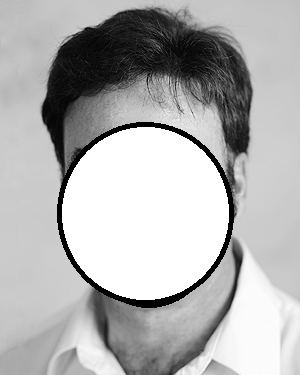
\includegraphics[width=1in,height=1.25in,clip,keepaspectratio]{author1.png}}]{First A. Author} received the B.S. and M.S. degrees in aerospace engineering from
the University of Virginia, Charlottesville, in 2001 and the Ph.D. degree in
mechanical engineering from Drexel University, Philadelphia, PA, in 2008.

From 2001 to 2004, he was a Research Assistant with the Princeton Plasma
Physics Laboratory. Since 2009, he has been an Assistant Professor with the
Mechanical Engineering Department, Texas A\&M University, College Station.
He is the author of three books, more than 150 articles, and more than 70
inventions. His research interests include high-pressure and high-density
nonthermal plasma discharge processes and applications, microscale plasma
discharges, discharges in liquids, spectroscopic diagnostics, plasma
propulsion, and innovation plasma applications. He is an Associate Editor of
the journal \emph{Earth, Moon, Planets}, and holds two patents.

Dr. Author was a recipient of the International Association of Geomagnetism
and Aeronomy Young Scientist Award for Excellence in 2008, and the IEEE
Electromagnetic Compatibility Society Best Symposium Paper Award in 2011.
\end{IEEEbiography}


\begin{IEEEbiography}[{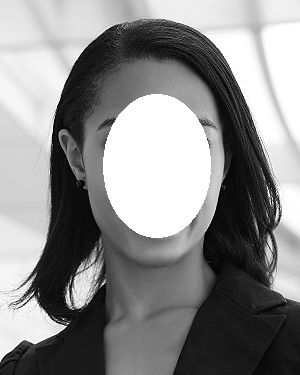
\includegraphics[width=1in,height=1.25in,clip,keepaspectratio]{author2.png}}]{Second B. Author} (M'76--SM'81--F'87) and all authors may include
biographies. Biographies are often not included in conference-related
papers. This author became a Member (M) of IEEE in 1976, a Senior
Member (SM) in 1981, and a Fellow (F) in 1987. The first paragraph may
contain a place and/or date of birth (list place, then date). Next,
the author's educational background is listed. The degrees should be
listed with type of degree in what field, which institution, city,
state, and country, and year the degree was earned. The author's major
field of study should be lower-cased.

The second paragraph uses the pronoun of the person (he or she) and not the
author's last name. It lists military and work experience, including summer
and fellowship jobs. Job titles are capitalized. The current job must have a
location; previous positions may be listed
without one. Information concerning previous publications may be included.
Try not to list more than three books or published articles. The format for
listing publishers of a book within the biography is: title of book
(publisher name, year) similar to a reference. Current and previous research
interests end the paragraph.

The third paragraph begins with the author's
title and last name (e.g., Dr.\ Smith, Prof.\ Jones, Mr.\ Kajor, Ms.\ Hunter).
List any memberships in professional societies other than the IEEE. Finally,
list any awards and work for IEEE committees and publications. If a
photograph is provided, it should be of good quality, and
professional-looking. Following are two examples of an author's biography.
\end{IEEEbiography}

\newpage

%If you do not have or do not want to include a photo, you can use IEEEbiographynophoto as shown below:

\begin{IEEEbiographynophoto}{Third C. Author, Jr.} (M'87) received the B.S. degree in mechanical
engineering from National Chung Cheng University, Chiayi, Taiwan, in 2004
and the M.S. degree in mechanical engineering from National Tsing Hua
University, Hsinchu, Taiwan, in 2006. He is currently pursuing the Ph.D.
degree in mechanical engineering at Texas A\&M University, College
Station, TX, USA.

From 2008 to 2009, he was a Research Assistant with the Institute of
Physics, Academia Sinica, Taipei, Taiwan. His research interest includes the
development of surface processing and biological/medical treatment
techniques using nonthermal atmospheric pressure plasmas, fundamental study
of plasma sources, and fabrication of micro- or nanostructured surfaces.

Mr. Author's awards and honors include the Frew Fellowship (Australian
Academy of Science), the I. I. Rabi Prize (APS), the European Frequency and
Time Forum Award, the Carl Zeiss Research Award, the William F. Meggers
Award and the Adolph Lomb Medal (OSA).
\end{IEEEbiographynophoto}

\EOD

\end{document}